
%%%%%%%%%%%%%%%%%%%%%%%%%%%%%%%%%%%%%%%%%%%%%%%%%%%%%%%%%
\section{Introducción a la mecánica de fluidos}
\subsection{Repaso de tensores cartesianos}
\[
a_i =\vec{a}= \begin{Bmatrix}
a_1 \\
a_2 \\
a_3
\end{Bmatrix}% \left\{ a_1,\; a_2, \; a_3\right\}
\]
\[
\gradient a_i=\nabla a_i = 
\begin{Bmatrix}
\vspace{.1cm}\spartial{a_1}{x_1} \\
\vspace{.1cm}\spartial{a_2}{x_2} \\
\spartial{a_3}{x_3}
\end{Bmatrix}%\left\{ \spartial{a_1}{x_1},\;\spartial{a_2}{x_2},\;\spartial{a_3}{x_3} \right\}
\]

\[
\diverg a_i = \nabla \cdot a_i=\nabla_k a_k=\partial_k a_k =\spartial{a_1}{x_1}+\spartial{a_2}{x_2}+\spartial{a_3}{x_3}
\]

\[
\rotor a_i = \nabla \times a_i  = -\epsilon_{ijk} \spartial{a_i}{x_j}= \epsilon_{ijk} \spartial{a_j}{x_i}
\]
El operador laplace:
\[
\nabla^2 a_i= \begin{Bmatrix}
\nabla^2 a_1 \\
\nabla^2 a_2 \\
\nabla^2 a_3
\end{Bmatrix} 
\]
donde
\[
\nabla^2 a = \dpartial{a}{x_1}+\dpartial{a}{x_2}+\dpartial{a}{x_3}=\frac{\partial^2 a}{\partial x_i \partial x_i} 
\]

La delta de Kronecker (matriz identidad):
\[
\delta_{ij}=\mathbf{I}=\begin{bmatrix}
1 & 0& 0\\
0 & 1 & 0\\
0 & 0 &1
\end{bmatrix}
\]
\subsection{Conceptos físicos básicos}
\subsubsection*{La materia}

Estados de agregación de la materia
\begin{itemize}
    \item Condensado de Bose-Einstein
    \item Sólido
    \item Liquido
    \item Gas
    \item Plasma 
\end{itemize}



Las fuerzas intermoleculares para moléculas de gas no-polares \citep{bird2002transport}: 

\[
F_r(r)=\frac{24 \epsilon}{r_{\min}}\left[ 2\left( \frac{r_{\min}}{r}\right)^{13} - \left( \frac{r_{\min}}{r} \right)^7 \right]
\]
dado por el \textit{potencial} $U_r$ \textit{de} \textit{Lennard-Jones}:
\[
U_r(r) = 4\epsilon \left[ \left(\frac{r_{\min}}{r}\right)^{12} - \left( \frac{r_{\min}}{r}\right)^6 \right] 
\]

En contraste a los sólidos, cuando un fluido recibe tensiones de corte, va tender a fluir. Por ende se puede inferir que un fluido en reposo \textbf{no} tiene tensiones de corte. 

Como toda materia consiste de moléculas, toda propiedad macroscópica puede ser descrita por propiedades moleculares pero, debido a la dificultades que surgen de un tratamiento molecular, se opta por la mecánica del continuo para describir propiedades del fluido\citep{durst2008fluid}. 
\subsubsection*{Modelo gas ideal}

Las leyes de los gases ideales están basadas en las leyes mecánicas para esferas que se mueven en el espacio \citep{durst2008fluid}.
\begin{itemize} 
    \item[Hip. I)] El volumen de los átomos y/o moléculas es extremadamente pequeño en comparación con la distancia entre ellos
    \item[Hip. II)] No hay fuerzas atractivas ni repulsivas ejercidas entre las moléculas excepto en el momento de choque
    \item[Hip. III)] Para la colisión entre dos moléculas, o una molécula y una pared, valen las leyes de colisiones perfectamente elásticas 
\end{itemize}

Ley para gases ideales:

\begin{equation} \label{eq:idealGasesLaw}
    \pe= \moldens \boltzmann T=\frac{N\overtilde{R}T}{V}
\end{equation}
donde $\boltzmann$ es la constante de Boltzmann y vale $\SI{1.380649e-23}{\meter \squared \kilogram \per \second \squared \per \kelvin}$. $\moldens$ es la cantidad de moléculas de gas por unidad volumen. $N$ es la cantidad de moles. $R$ es la constante de gas ideal universal $\overtilde{R}=\SI{8,31447}{\joule \per \mole \per \kelvin}$. $\pe$ es la \textbf{presión termodinámica}

Existe también la expresión especifica de la ley para gases ideales
\[
\pe = \frac{RT}{v} = \rho R T
\]
donde $v=\frac{1}{\rho}$ es el volumen especifico y  $R$ [\si{\joule \per \kilogram \per \kelvin}] es la constante especifica del gas.

Generalmente el contenido de energía de un gas ideal está dado por
\begin{equation}
    e_{gas}=\frac{\alpha}{2}\boltzmann T
\end{equation}
donde $\alpha$ indica los grados de libertad del movimiento molecular. $\alpha=3$ para gases monoatómicos, $\alpha=5$ para gases diatómicos y $\alpha=6$ para gases triatómicos y poliatómicos.

En el estado gaseoso las moléculas tienen un movimiento aleatorio cuya velocidad promedio puede dar cero, pero la velocidad cuadrática media viene dada por
\[
\langle U^2 \rangle = \frac{3\overtilde{R}T}{M} \Rightarrow \quad U_{cm}=\sqrt{\frac{3\overtilde{R}T}{M}}
\]

\subsection{Modelo continuo}
Partimos definiendo un volumen de forma de cubo en nuestro fluido de lado $\Delta$ tal que su volumen es $\Delta^3$. La \textbf{densidad}  dentro de nuestro cubo virtual está dado por $\rho_\Delta$ 
\[
\rho_\Delta = \frac{m\cdot N_\Delta}{\Delta^3} \quad \textrm{en} \quad [\si{\kilogram \per \meter \cubed}]
\]
donde $m$ es la masa de una sola molécula, $N_\Delta$ es la cantidad de moléculas en el cubo virtual mencionado anteriormente.

Si partimos de un tamaño muy pequeño tendremos que varía mucho la densidad de moléculas en nuestro cubo. Mientras aumentamos $\Delta$ irá disminuyendo la variación hasta que sea cuasi-constante el valor de $\rho_\Delta$. 

\subsubsection*{Camino libre entre moléculas}
La materia podrá suponerse un continuo cuando $K_n\lesssim 0,1$ (Número de Knudsen)
\[
K_n = \frac{\lambda}{L}
\]
donde $\lambda$ es el camino libre medio entre colisiones y $L$ es la dimensión lineal característica.\footnote{Diámetro del tubo, ancho de caja etc.}

El camino libre medio $\lambda$ se puede calcular con la expresión
\[
\lambda = \frac{1}{\sqrt{2} \pi d^2 \moldens}
\]
donde $d$ es el diámetro molecular y $\moldens$ la densidad de partículas en un volumen. $\moldens$ es proporcional a $\frac{p}{T}$ luego $\lambda \propto \frac{T}{p}$

Para el aire tenemos $\moldens \approx \num{2,5e25}$, $d\approx \num{4e-10}$ según fuentes on-line $\Rightarrow \lambda_{\textrm{aire}} \approx \SI{5,6e-8}{\meter}=56\si{\nano \meter}$
\begin{mdframed}
A partir de aquí se comienza el tratamiento \textit{continuo} del fluido. Es decir, toda expresión consiguiente vale para volúmenes de control donde la longitud característica ceda $K_n \lesssim 0,1$!
\end{mdframed}

\subsection{Tensiones}
Las componentes de $\ttens{\sigma}$ (o $\sigma_{ij}$) representan la componente $i$ que aparece sobre una superficie orientada por el vector normal $n_j$ a esa superficie. Las fuerzas por unidad de superficie $\underline{f}$ están dadas por:
\[
\underline{f}=
\begin{Bmatrix}
f_1 \\
f_2 \\
f_3
\end{Bmatrix} =
\begin{bmatrix}
\sigma_{11} & \sigma_{12} & \sigma_{13} \\
\sigma_{21} & \sigma_{22} & \sigma_{23} \\
\sigma_{31} & \sigma_{32} & \sigma_{33} \\
\end{bmatrix} \cdot
\begin{Bmatrix}
n_1 \\
n_2 \\
n_3
\end{Bmatrix}
\]

El tensor de esfuerzos se puede separa en su parte isótropa (hidrostática) $\ttens{\sigma}^H$ y no isótropa (o desviadora) $\ttens{S}$ tal que $\ttens{\sigma}=\ttens{\sigma}^H+\ttens{S}$ con
\[
\sigma_{ij}^H=\sigma_m \cdot \begin{bmatrix}
1 & 0 & 0 \\
0 & 1 & 0 \\
0 & 0 & 1
\end{bmatrix}
\]
donde $\sigma_m = \frac{1}{3}\sigma_{kk}$ y 

\[
S_{ij}= \begin{bmatrix}
\sigma_{11}-\sigma_m & \sigma_{12} & \sigma_{13} \\
\sigma_{21} & \sigma_{22}-\sigma_m & \sigma_{23} \\
\sigma_{31} & \sigma_{32} & \sigma_{33}-\sigma_m 
\end{bmatrix}
\]

Cabe destacar que $\ttens{\sigma}^H$ contempla las componentes normales y está asociado al equilibrio del fluido mientras que $\ttens{S}$ se relaciona a los esfuerzos tangenciales y está asociado a un gradiente de velocidades. Se los suele denominar el \textbf{tensor hidrostático} y el \textbf{tensor de desviaciones}, respectivamente. 

La presión mecánica se define como $p=-\sigma_m$. Si el sistema está en equilibrio (mecánico y termodinámico) entonces $p$ resulta ser la presión termodinámica. Si $\ttens{S}=\pmb{0}$ se puede inferir que el fluido está en equilibrio hidrostático ($p=\pe$), pero no necesariamente en reposo.
 \label{sec:presionmecanica}
 

\subsection{Reología} \label{sec:reologia}
La reología es la rama de la física encargada del estudio de la deformación y flujo de la materia. Para un fluido newtoniano con solo una componente de velocidad $U_q$ se puede definir
\begin{equation}
    \tau_{pq}=-\mu \spartial{U_q}{x_p}
\end{equation}
donde $\mu$ es la \textbf{viscosidad dinámica}, $p$ indica la dirección del transporte molecular (normal a la velocidad [ver nota \ref{foot:transporteMolecular}]) y $q$ indica el componente de velocidad.

En general para fluidos
\begin{equation}
    \tau_{ij}=-\mu \left( \spartial{u_j}{x_i}+\spartial{u_i}{x_j}\right) -\lambda \delta_{ij} \spartial{u_k}{x_k}
\end{equation}
donde $\lambda$ es conocida como la \textit{segunda viscosidad}, \textit{viscosidad de expansión/dilatación} o viscosidad de volumen \citep{durst2008fluid}. Para resolver problemas de fluidos no se suele disponer del valor de $\lambda$. Para gases ideales monoatómicos $\lambda \equiv 0$ y si se trabaja con un flujo incompresible entonces se tiene que $\spartial{u_k}{x_k}=0$ y por lo tanto el término asociado es cero. La segunda viscosidad es importante para el comportamiento de gases poliatómicos ante vibraciones de altas frecuencias (absorción de ruido) y cuando se quiere describir un liquido con burbujas.

\begin{itemize}
    \item Para los gases: $\mu$ aumenta con el aumento de la temperatura
    \item Para los líquidos: $\mu$ disminuye con el aumento de la temperatura
\end{itemize}
\subsubsection*{Explicación viscosidad}
Los términos de $\tau_{ij}$ usados en mecánica de fluidos \textbf{no son} considerados como a causa de fricción \citep{durst2008fluid}! 

La viscosidad se puede describir como un intercambio de masa al nivel molecular\footnote{Dicho intercambio se suele denominar \textbf{transporte molecular.} \label{foot:transporteMolecular}} entre dos capas de un fluido que se mueven a distintas velocidades en el mismo sentido. Por consecuencia de esta diferencia de velocidades entre capas, dicho proceso conlleva también un \textbf{intercambio de cantidad de movimiento}. La capa mas rápida se \textit{desacelera} y la mas lenta se \textit{acelera} en dirección de la velocidad del flujo. De aquí surgen las ``tensiones"{} tangenciales.\footnote{Más que tensiones, $\tau_{ij}$ representa el transporte de cantidad de movimiento por unidad de área por unidad de tiempo.}


\subsubsection*{Relación constitutiva}
La relación constitutiva para fluidos de interés industrial con comportamiento \textit{independiente del tiempo} esta dada por

\[
\sigma_{ij}=\sigma_0+K\dot{\gamma}_{ij} \left| \dot{\gamma}_{ij}\right|^{n-1}
\]
donde $\sigma_0$ es la tensión de fluencia\footnote{Para fluidos del tipo plástico real y Bingham}, $K$ es denominado el índice de consistencia, $n$ es el índice reológico\footnote{$n=1$ para fluidos newtonianos y Bingham. Si $n>1$ el fluido es dilatante. Si $n<1$ el fluido es plástico.} y $\dot{\gamma}$ es la velocidad de deformación tal que $\dot{\gamma}_{ij}=\frac{1}{2}\left( \spartial{u_i}{x_j}+\spartial{u_j}{x_i}\right)$. Luego, en las secciones \ref{sec:CinematicaDeElementosdeFluido} y \ref{sec:NewtonTTR}, se definirá (y se hallará por ``casualidad", respectivamente) un tensor idéntico $e_{ij}$.

Se define la \textbf{viscosidad aparente} como $\eta$ y depende de la velocidad de deformación\footnote{Para fluidos no-newtonianos.} y del estado termodinámico ($p,T$).
\[
\eta=K\left| \dot{\gamma} \right|^{n-1}
\]
para fluidos newtonianos $K$ es constante y vale dos veces las \textbf{viscosidad dinámica}: $K=2\mu$.

\begin{figure}[htb!]
	\centering
	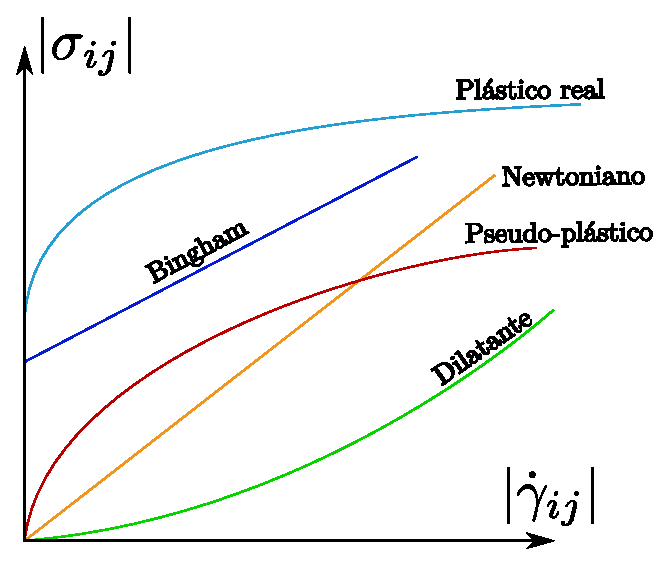
\includegraphics[width=.49\textwidth]{fig/deformacion-tensionFluidos.eps}
	\caption{Gráfico tensión-velocidad de deformación para un fluido newtoniano y varios no-newtonianos.}
\end{figure}

\derpq Alguna vez quisiste servir kétchup que tardaba en salir de la botella al principio y después de unos segundos salía a los chorros? 

Esto es un ejemplo de comportamiento \textbf{dependiente del tiempo}.\footnote{Cabe destacar que el comportamiento dependiente del tiempo es característica no-newtoniana pero no todos los fluidos no-newtonianos son dependientes del tiempo.} Para estos fluidos la viscosidad aparente depende del tiempo durante el cual el fluido es sometido a esfuerzo. La viscosidad de los fluidos \textbf{tixotrópicos} disminuye con el tiempo (kétchup) y para los \textbf{reopécticos} aumenta con el tiempo.

\subsection{Tensión superficial}
Así como hay fuerzas que actúan sobre volumen $F_\smol{V}=\rho g\cdot V$ (gravedad) y superficie $F_\smol{S}=p\cdot S$ (presión), existen fuerzas que actúan sobre \textit{longitudes}. Para el caso de los fluidos, es la \textbf{tensión superficial}. Esta fuerza la solemos despreciar en nuestro día a día, pero cuando se tienen sistemas microscópicos, esta fuerza domina.
\[
F_\smol{L} = \Upsilon L
\]%fighere
donde $\Upsilon$ (Ípsilon) es una propiedad del interfaz entre el liquido y el gas. $\Upsilon$ también depende de las propiedades termodinámicas de los fluidos. Para agua en contacto con aire a CNPT $\Upsilon=\SI{7,28e-2}{\newton \per \meter}$.

Comparamos un volumen dado por un cubo ``pequeño'' de 1mm de lado con otro ``grande'' de 1m. Para el cubo pequeño
\vspace{-.2cm}
\[V_p=1\si{\milli \meter \cubed},\, S_p=6 \si{\milli \meter \squared},\, L_p = 12 \si{\milli \meter} \]
y para el cubo grande tenemos
\vspace{-.2cm}
\begin{gather*}
    V_g=\SI{1e9}{\milli \meter \cubed},\, S_g=\SI{6e6}{\milli \meter \squared},\\ L_g =\SI{12e3}{\milli \meter}
\end{gather*}
con esto resulta aparente que la relación de fuerzas $\frac{F_\smol{L}}{F_\smol{V}}$ disminuye fuertemente con el aumento del tamaño característico del problema. Para el rango de número de Bond $\Bond \lesssim 1$ se tiene que las fuerzas capilares son apreciables en comparación con la gravedad. La longitud característica $L_c$ a la cual el número de Bond es uno se denomina la longitud capilar. $\Bond_{L_c}=1$

Un efecto de superficie importante es el ángulo de contacto $\theta$ medido desde el seno del fluido al ángulo que forma sobre la superficie, que aparece cuando un liquido entra en contacto con una superficie solida y otro fluido. El balance de fuerzas se realiza tomando en cuenta los parámetros $\Upsilon$ y $\theta$. Sí $\theta<90\grados$ entonces el liquido moja la superficie; sí $\theta>90\grados$ entonces el liquido no moja.%fighere

\subsubsection{Inestabilidad en chorros libres pequeños}
Los sistemas tienden al estado de menor energía. Para un chorro libre de $\Bond_R \lesssim 1$ los efectos de tensión superficial hacen que se formen gotas. Tomando un volumen de control sobre un chorro cilíndrico y planteando su superficie expuesta al medio y la superficie de un sistema de $n$ gotas de igual volumen se puede demostrar que se \textit{reduce la energía del sistema para un radio} $r$ \textit{de gota}:
\begin{gather*}
	V_{\mathrm{cil.}}=V_{\mathrm{esf.}} \Rightarrow	\pi R^2 L =n \frac{4}{3}\pi r^3 \\
	S_{\mathrm{cil.}}=2\pi RL, \qquad S_{\mathrm{esf.}}=n4\pi r^2
\end{gather*}
se analiza el caso más favorable en donde todo el fluido del cilindro es juntado en una esfera, maximizando la reducción de superficie y por ende su energía. Con esta consideración se tiene que cumplir $r>\frac{3}{2}R$ para que la gota reduzca la energía del sistema. 


\subsection{Cavitación}
El fenómeno de la cavitación se refiere a la rápida formación \textit{y colapso} de burbujas de vapor en un liquido. Ocurre cuando la presión termodinámica es menor a la presión de vapor. Es importante en el diseño de aspas para bombas y hélices de barcos ya que la presencia de la cavitación daña los componentes cercanos a la implosión de las burbujas.

\subsection{Cinemática de elementos del fluido} \label{sec:CinematicaDeElementosdeFluido}
Los elementos de un fluido pueden sufrir tres tipos de movimientos cinemáticos dado un campo de velocidades $u_i$ 
\begin{itemize}
    \item Traslación
    \item Rotación
    \item Deformación
\end{itemize}

Para un fluido \textbf{rotacional} el rotor nos cede la \textit{vorticidad} $\xi_k$ igual al doble de la velocidad angular $\omega_k$ del elemento del fluido sobre su eje central.
\begin{equation}
    \rotor u_i =\epsilon_{ijk}\spartial{u_i}{x_j}=\xi_k= 2\omega_k 
\end{equation}
Sí $\omega_k$ vale cero entonces el fluido es \textbf{irrotacional}. 

La \textit{razón de deformación} $e_{ij}=\dot{\gamma}_{ij}$ está asociada a la elongación o deformación de ángulos. \begin{equation}
    e_{ij}=\frac{1}{2}\left( \spartial{u_j}{x_i}+\spartial{u_i}{x_j}\right)
\end{equation}

Considere una curva cerrada $C$ en un campo de velocidades $u_j$. La \textit{circulación} instantánea alrededor de la curva $C$ está dada por una integral de linea donde $s_k$ es el vector tangencial a $C$
\begin{equation}
    \Gamma \equiv - \oint_C u_k s_k \di \ell
\end{equation}
por el teorema de Stokes podemos llegar a relacionar la vorticidad con la circulación
\[
\Gamma \equiv\! -\! \oint_C\!\! u_k s_k \di \ell =\! -\!\iint_S \left( \rotor u_k \right)n_k\di \sur=\! -\!\iint_S\! \xi_k n_k\di \sur
\]
flujos irrotacionales (por definición $\xi=0$) por ende tienen $\Gamma=0$. Típicamente los flujos aerodinámicos son de este tipo. La única restricción a este principio general es que el contorno tiene que ser reducible a un punto dentro del campo de flujo. Un álabe es un ejemplo de un contorno no reducible con $\Gamma>0$ \citep{durst2008fluid}.
\subsubsection{Principio de no-deslizamiento}
Para el estudio ingenieril de flujos en proximidad de paredes se aplica la condición de velocidad \textit{relativa} nula del fluido sobre el interfaz solido-fluido, paralelo a la linea de borde. Esto quiere decir que el fluido se moverá a la velocidad del solido.

Cabe destacar que para problemas con tamaños característicos pequeños (del orden de la longitud de camino libre $\lambda$) habrá deslizamiento. Para dicho caso se puede calcular la velocidad de deslizamiento
\[
u_{\textrm{deslizamiento}}=u-u_s=\beta \spartial{u}{n}
\]
donde $\beta$ es la longitud de deslizamiento\footnote{Se puede aproximar con una proporción del camino libre medio: $\beta\approx 1,15\lambda$ para gases.} y $n$ es la dirección normal a la superficie.

\subsubsection{Flujo laminar}
El flujo laminar se caracteriza por fluir en capas sin mezclarse y su campo de velocidades depende de solo una componente la cual es perpendicular a la dirección del flujo. El flujo laminar ocurre a número de Reynolds relativamente bajos debido a uno de los siguientes
\begin{itemize}
    \item Velocidad baja
    \item Viscosidad alta
    \item Densidad baja
    \item Longitud característica pequeña
\end{itemize}

Una vez que el número de Reynolds es lo suficientemente alto, comienza la turbulencia. Cada caso tiene su número de Reynolds crítico $\Reynolds_\crit$ al cual comienza el régimen de transición que lleva a la turbulencia. Abajo se tienen algunos casos listados
\begin{itemize}
    \item Flujo en un caño $\Reynolds_\textrm{trans.}=2700\mhyph5000$
    \item Flujo alrededor de un cilindro $\Reynolds_\crit \approx \num{3e5}$
\end{itemize}

\subsection{Diferencia entre líquidos y gases}
A diferencia de los gases, los líquidos no presentan un cambio apreciable de volumen cuando se les aplica una presión. Se puede suponer entonces que los líquidos \textbf{\textit{en reposo}} son incompresibles. Recordar que la incompresibilidad no es una propiedad del fluido, si no del flujo. Es decir, un flujo de gas puede comportarse de manera incompresible bajo ciertas condiciones.

%%%%%%%%%%%%%%%%%%%%%%%%
%%   FLUIDOSTATICA    %%
%%%%%%%%%%%%%%%%%%%%%%%%

\section{Fluidostática}
\subsection{Ecuación de fluidostática}
Partimos de balancear las fuerzas de un elemento de fluido \textit{estático} de volumen arbitrario $V$ con superficie $S$. Nos adelantamos a la sección \ref{sec:NewtonTTR}, ecuación \ref{eq:ttrp} donde $B_j$ son las fuerzas por unidad de volumen y $b_j=\frac{B_j}{\rho}$ son las fuerzas por unidad de masa:
\[
\sum F_j = \int_V B_j \di \vol + \int_S \sigma_{ij} n_i \di \sur
\]
considerando que el fluido esta en reposo y en equilibrio se llega a que $\sigma_{ij}=-\pe \delta_{ij}+\cancel{S_{ij}}$ y $\sum F_j=\vec{0}$. De aquí en adelante para la sección de fluidostática la presión de equilibrio será igual a la mecánica, la llamamos simplemente $p$.
\[
0=\int_V \rho b_j \di \vol + \int_S -p\delta_{ij}n_i \di \sur
\]

El teorema de la divergencia de Gauss nos ayuda
\[
\int_S -p\delta_{ij}n_i \di \sur = \int_V -p \delta_{ij}\partial_i \di \vol
\]
Entonces:
\[
0=\int_V \left(\rho b_j - p\delta_{ij}\partial_i\right) \di \vol
\]
como se definió para un volumen arbitrario, lo de adentro del integrando debe ser igual a cero. Así llegamos a la ecuación de la fluidostática
\begin{equation} \label{eq:fluidostatica}
    \rho b_j = \spartial{p}{x_j}
\end{equation}

\subsubsection*{Demostración}
\textit{Demostrar que las curvas isobaras son colineales a las equipotenciales de las fuerza por unidad de masa.}

Si $b_j$ es conservativa entonces existe una función potencial $\varphi$ tal que $\partial_j \varphi =b_j$. Entonces:
\[
\spartial{}{x_j}\left(\rho \varphi +p \right) = 0
\]
integrando respecto una dirección arbitraria llegamos a que $\rho \phi+p=\textrm{constante}$, por ende, si $\varphi$ es constante entonces $p$ también es constante.

\subsubsection*{La atmósfera}
Aproximando el aire como un gas ideal y tomando en cuenta que el perfil de temperaturas en la troposfera está dado aproximadamente por $T\approx T_0 -B z$ podemos obtener la presión a una dad altura resolviendo \eqref{eq:fluidostatica} y $p=\rho R T$ simultáneamente
\[
 \frac{\di p}{\di z}=\rho( -g) =-g\left(\frac{p}{RT}  \right) 
\]
integrando desde el nivel del mar $p_0,z_0=0$ para arriba:
\[
\ln \frac{p}{p_0}= \frac{g}{B\cdot R} \ln\left(\frac{T_0-Bz}{T_0-B(0)}\right) 
\]
nos queda que la presión a una altura $z$ esta dada por la ecuación:
\[
p(z) = p_0 \left( 1-\frac{Bz}{T_0}\right)^{\frac{g}{BR}}
\]
donde para aire (constante especifica del aire) $R_{\textrm{aire}}=\SI{287}{\meter \squared \per \second \squared \per \kelvin}$.

Suponiendo una atmósfera isotérmica se puede prescindir del valor $B$ (según acuerdo internacional $B=\SI{6,50e-3}{\kelvin \per \meter}$ y  $T_0\approx 288 \si{\kelvin}$).

\newcommand{\CP}{{\mbox{\tiny $C\!P$}}}
\newcommand{\CG}{{\mbox{\tiny $C\!G$}}}
\subsection{Compuertas}
\subsubsection*{Compuertas sumergidas planas}
La fuerza ejercida sobre una compuerta esta dado por
\begin{equation}
F=p_{\CG}A_{moj}
\end{equation}
donde $p_{\CG}$ es la presión absoluta en el centroide del área ``mojada"{} de la compuerta y $A_{moj}$ es el área mojada. $F$ actúa normal a la superficie de la compuerta plana.

Esta fuerza actúa sobre el centro de presiones, el cual esta desplazado\footnote{El sistema $x$ e $y$ esta contenido dentro del plano de la compuerta (plana)} del centroide según

\begin{gather}
y_{\CP} = -\frac{\rho g I_{xx}}{p_{\CG}A_{moj}} \\
x_{\CP} = - \frac{\rho g I_{xy}}{p_{\CG}A_{moj}}
\end{gather}
donde $I_{xx},I_{xy}$ son los momentos de inercia de la forma geométrica de la compuerta proyectada en dirección $x$.

\subsubsection*{Compuertas sumergidas curvas}
Ayuda descomponer la fuerza en dos direcciones, una siendo en la dirección de la aceleración
%%%%%%%%%%%%%%%%%
%%  BERNOULLI  %%
%%%%%%%%%%%%%%%%%

\section{Ecuación de Bernoulli}
\subsection{Bernoulli sin perdidas}
Las hipótesis para aplicar Bernoulli \textbf{sin pérdidas}:
\begin{itemize}
    \item[H1)] Flujo en régimen estacionario
    \item[H2)] Flujo incompresible (Número de Mach $\Mach<0,3$)
    \item[H3)] Flujo sin pérdidas por fricción (invíscido)
    \item[H4)] Flujo unidimensional ($\alpha=1$)
\end{itemize}
con las hipótesis anteriores se puede aplicar la ecuación de Euler (sección \ref{sec:NewtonTTR}) a un volumen de control y así obtener la ecuación de Bernoulli sin perdidas:
\begin{gather*}
    \frac{p_2-p_1}{\rho}+\tfrac{1}{2}(U_2^2-U_1^2)+g(z_2-z_1)=0\\
    p_1+\tfrac{1}{2}\rho U_1^2+\rho gz_1=p_2+\tfrac{1}{2}\rho U_2^2+\rho g z_2=\textrm{const}
\end{gather*}
donde los puntos $1$ y $2$ quedan sobre la \textbf{misma linea de flujo.} En el caso que el flujo sea \textbf{irrotacional}, esta última condición no es necesaria y hay una altura de Bernoulli para todo el flujo.

Dado que supusimos que el flujo es unidimensional no es del todo correcto aplicar el principio de no deslizamiento. La diferencia entre las mediciones (figura \ref{fig:diagramaBernoulli}) es para mejor visualizar lo que ocurre en la siguiente sección para Bernoulli generalizada. 

\begin{figure}
    \centering
    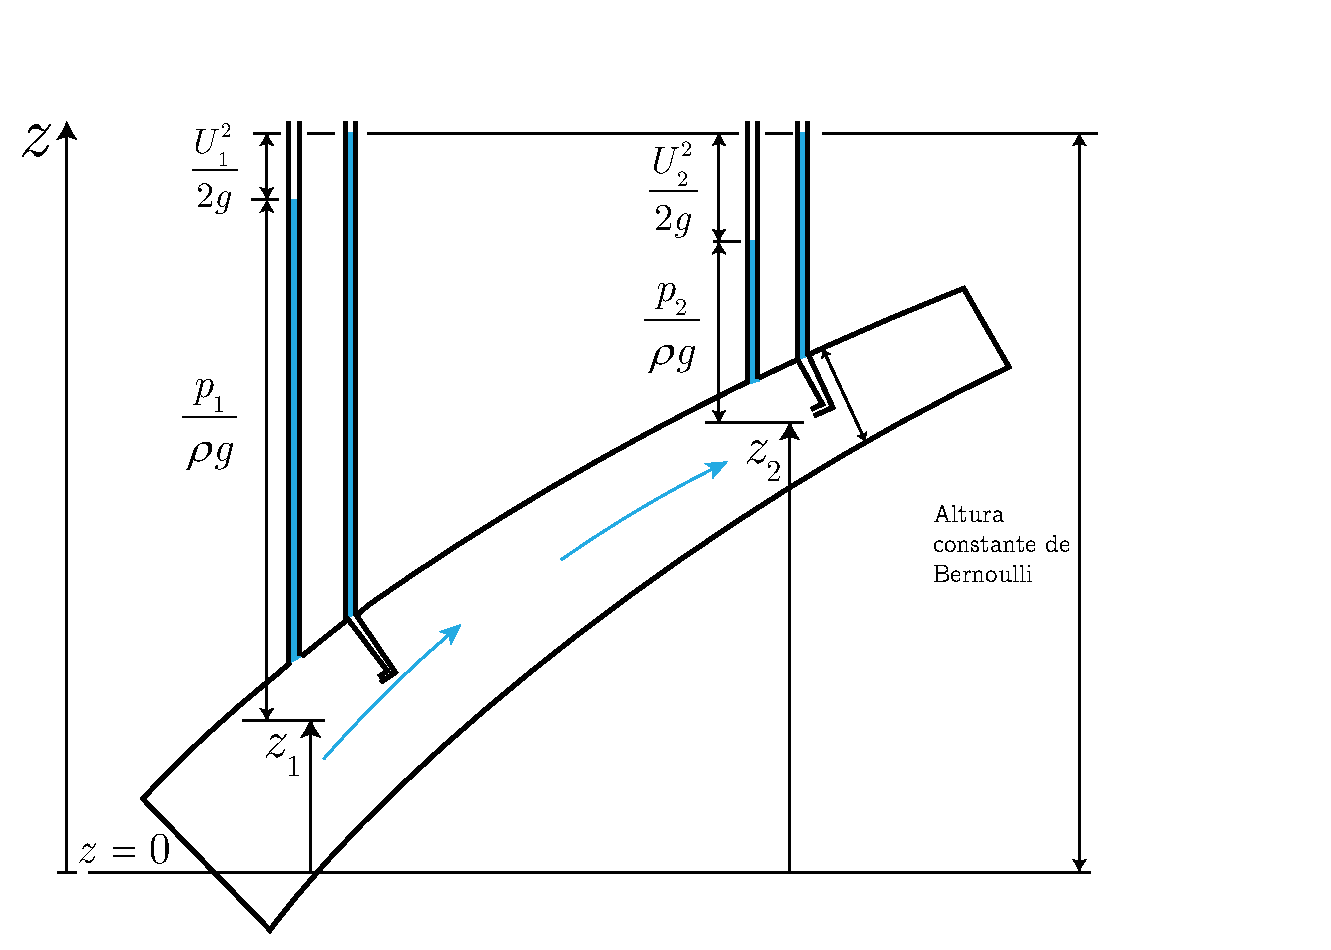
\includegraphics[width=.5\textwidth]{fig/bernoullidiag.eps}
    \caption{Visualización de la ecuación de Bernoulli \underline{sin pérdidas} en un caño que se va achicando en sección. Notar la diferencia entre la medida de un piezómetro y un tubo de pitot (ver condición de no-deslizamiento).}
    \label{fig:diagramaBernoulli}
\end{figure}
\subsection{Bernoulli generalizada}
Bernoulli con pérdidas, tomando en cuenta el perfil de velocidades (flujo bidimensional), siempre planteando el punto 1 del volumen de control ``aguas arriba":
\begin{equation}\label{eq:bernoulliPerdidas}
    \overbrace{\frac{\dot{W}}{gQ\rho}}^{I}+\overbrace{\frac{p_1}{g\rho}}^{II}+\overbrace{\frac{\alpha_1 U_1^2}{2g}}^{III}+\overbrace{z_1}^{IV}=\frac{p_2}{g\rho}+\frac{\alpha_2 U_2^2}{2g}+z_2+\overbrace{h_p}^{V}
\end{equation}
\begin{itemize}
    \item[I.] Altura relacionada al trabajo $\dot{W}$ hecho por bomba(s) o reacción química. Es igual a la altura $H_{\RM{B}}$ referida en el próxima sección
    \item[II.] Altura relacionada a la presión estática
    \item[III.] Altura relacionada a la presión dinámica
    \item[IV.] Altura de referencia del punto 1 del volumen de control tomado
    \item[V.] Altura de las pérdidas
\end{itemize}
donde $Q$ [\si{\meter \cubed \per \second}] es el caudal y $h_p$ es la altura de las pérdidas entre los puntos $1$ y $2$. 
\subsubsection*{Factor de correción a la energía $\alpha$}
El número $\alpha_1$ es un factor de corrección para la energía cinética que relaciona la velocidad media $U_1$ con el perfil de velocidades en el tubo. En régimen laminar $\alpha_{\textrm{laminar}}=2,0$. Para flujo turbulento con perfil del tipo
\[
U(r)=U_0 \left(1-\frac{r}{R}\right)^{m}
\]
donde $m$ suele variar entre $\frac{1}{5}$ y $\frac{1}{9}$
\[
\alpha_{\textrm{turb.}}=\frac{(1+m)^3(2+m)^3}{4(1+3m)(2+3m)}
\]
en general se suele tomar $\alpha_{\textrm{turb.}}=1,0$ para análisis elemental ya que este varía entre $\alpha_{\textrm{turb.}}\approx 1,04\mhyph1,11$.

\subsubsection*{Altura de las pérdidas $h_p$}
\vspace{-.75cm}
\begin{equation} \label{eq:alturaPerdidas}
    h_p=\overbrace{\sum^{n_L}_\iota \frac{U_\iota}{2g} \cdot \bigg(f_\iota\frac{L_\iota}{D_\iota}\bigg)}^{I}+\overbrace{\sum^{n_K}_\kappa \frac{U_\kappa}{2g} \cdot \big(K_\kappa\big)}^{II}
\end{equation}
donde $f$ es el \textit{factor de fricción de Darcy} y está en función del diámetro de la tubería ($D$), la rugosidad de las paredes de la tubería ($\epsilon$) y el número de Reynolds ($\Reynolds_D$). $L$ es la longitud del trayecto con pérdidas distribuidas. El término asociado con las perdidas \underline{no} va acompañado con un factor de corrección $\alpha$. 
\begin{itemize}
    \item[I.] Término relacionado a las pérdidas distribuidas
    \vspace{-.2cm}
    \item[II.] Término relacionado a las pérdidas localizadas
\end{itemize}
La razón por la cual se expresan las pérdidas como una sumatoria es porque a lo largo del trayecto el tubo puede cambiar de diámetro, y por lo tanto, también de velocidad. Cada pérdida tiene que ser calculada con su velocidad correspondiente, sea distribuida o localizada.

%%%%%%%%%%%%
%% BOMBAS %%
%%%%%%%%%%%%
\subsection{Instalaciones con bombas}

Cada bomba centrifuga tiene su curva característica caudal $Q$ versus altura $H_{\RM{B}}$. Esta se puede aproximar con una cuadrática de aspecto
\begin{equation}
    H_{\RM{B}} = A_{\RM{B}}+B_{\RM{B}} Q^2
\end{equation}
donde $A_{\RM{B}}$ y $B_{\RM{B}}$ son constantes que se pueden obtener del fabricante.

Un ingeniero suele estar interesado en si es apta una bomba para una instalación. Para que lo sea se tiene que verificar:
\begin{itemize}
    \item Existe una intersección de la curva de demanda (curva del sistema) con la curva de la bomba $H_{\RM{B}} = H_{\RM{S}}$
    \item No hay cavitación en ningún punto de la instalación
\end{itemize}
luego se podría verificar si el caudal que circula es suficiente para refrigerar la bomba correctamente o si se requiere más caudal para los propósitos del sistema.

La curva del sistema se obtiene planteando Bernoulli entre el punto de aspiración y de descarga.

\[
H_{\RM{S}}+\frac{p_a}{g\rho}+\frac{\alpha_aU_a^2}{2g}+z_a =\frac{p_d}{g\rho}+\frac{\alpha_d U_d^2}{2g}+z_d+h_p
\]
aquí tenemos el caudal camuflado en el término de la velocidad. Despejando y sabiendo que $U^2=\frac{Q^2}{(\pi D^2/4)^2}$

\begin{equation}
H_{\RM{S}} = A_{\RM{S}}+B_{\RM{S}}Q^2
\end{equation}
donde
\begin{gather*}
A_{\RM{S}} = \frac{p_d-p_a}{g\rho}+z_d-z_a \\
B_{\RM{S}} = \frac{8\alpha_d}{\pi^2gD_d^4}-\frac{8\alpha_a}{\pi^2gD_a^4}+\sum_k^n\frac{8}{\pi^2gD_k^4}\cdot\left(f_k\frac{L_k}{D_k}+K_k \right)
\end{gather*}
\newcommand{\Qstar}{{Q^{*}}}

Igualando $H_{\RM{B}}$ a $H_{\RM{S}}$ se obtiene el caudal que circularía si se instalara la bomba. Este caudal se suele escribir como $\Qstar$.\footnote{Aquí se agruparon las sumas de \eqref{eq:alturaPerdidas} para más claridad.}

\subsubsection*{El ANPA}
El \textbf{ANPA} (NPSH en inglés) es la Altura Neta Positiva de Aspiración. Es dada por el fabricante de la bomba e indica la caída de presión, en metros de columna de agua, entre la entrada de la bomba y la aspa en el interior. Se usa para verificar que no se produzca el fenómeno de la cavitación dentro de la bomba, pues esta puede ocasionar daños severos. Si no se cumple la siguiente igualdad hay peligro de cavitación:

\begin{equation} \label{eq:ANPA}
    \frac{p_{\entrada}}{\rho g} - ANPA - M_s > \frac{p_v(T)}{\rho g}
\end{equation}
donde $p_\entrada$ es la presión a la entrada de la bomba, $M_s$ es el margen de seguridad\footnote{Puede tomarse como 5 metros.} y $p_v(T)$ es la presión de vapor del liquido bombeado, el cual depende de la temperatura! 

Atento a los siguientes casos que comprometen la bomba:
\begin{itemize}
    \item Pérdidas altas en aspiración
    \begin{itemize}
        \item Tuberías angostas en aspiración
        \item Válvulas/filtros en aspiración
    \end{itemize}
    \item Bomba elevada sobre el nivel del fluido aspirado
\end{itemize}
\subsection{Turbulencia en caños}
Un lector ávido tal vez recuerde que $f$ está en función de $\Reynolds_D$. Esto no es un problema \textit{demasiado} grave en régimen Laminar pues $f_{\textrm{laminar}}=\frac{64}{\Reynolds}$. En régimen turbulento sobran problemas numéricos...  Iterando sobre diferentes valores de $Q$ se obtienen valores de $\Reynolds_D$ y $f$ con la siguiente ecuación
\begin{equation} \label{eq:darcyExact}
    \frac{1}{\sqrt{f}}=-2\log \left[ \frac{\epsilon/D}{3,7}+\frac{2,51}{\Reynolds_D \sqrt{f}} \right]
\end{equation}
si uno no tiene ganas de resolver dado problema numérico puede usar una aproximación:
\[
\frac{1}{\sqrt{f}}\approx -1,8\log \left[ \left(\frac{\epsilon/D}{3,7}\right)^{1,11}+\frac{6,9}{\Reynolds_D}\right]
\]
también se tienen diversos diagramas de Moody a disposición del ingeniero (Ver figura \ref{fig:moodydiagram}).
\begin{figure}[htb!]
    \centering
    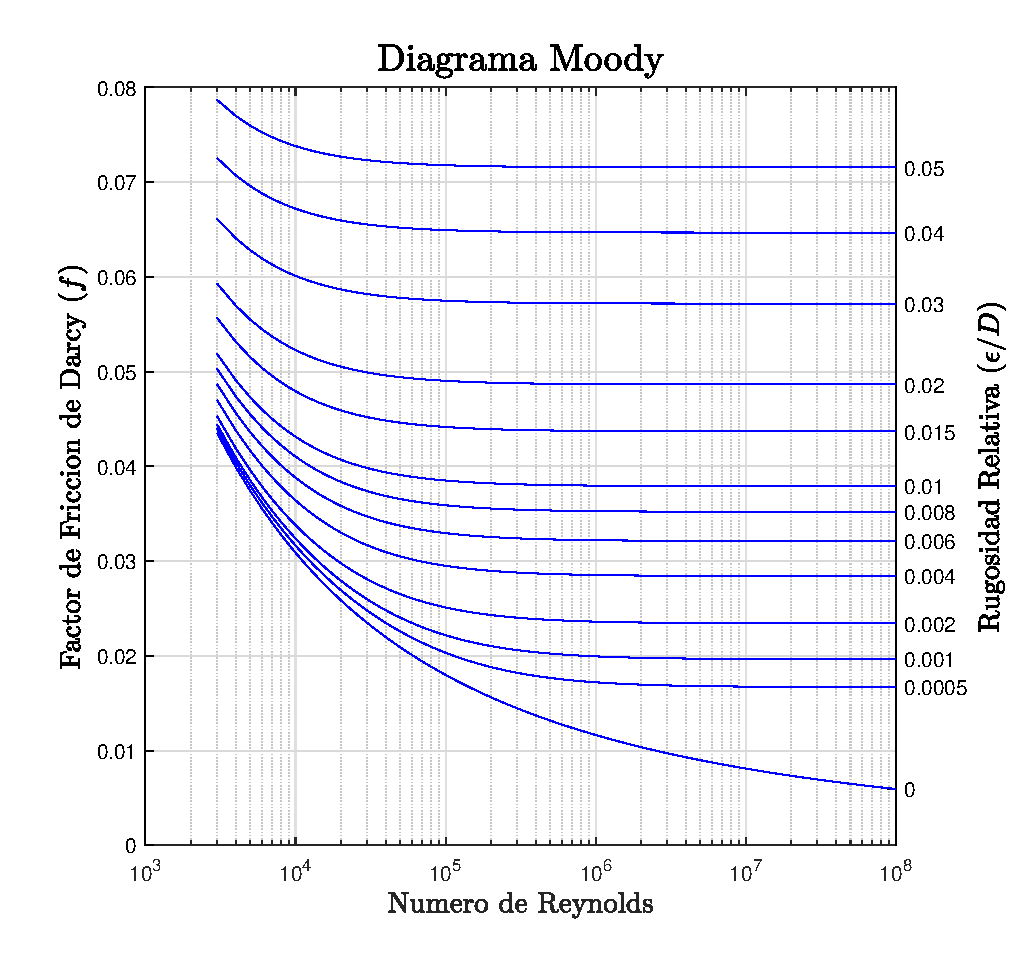
\includegraphics[width=0.475\textwidth]{fig/moodydiag.eps}
    \caption{Graficado y resuelto numéricamente en \Matlab. Observe como a grandes Reynolds $f$ es constante para una dada rugosidad relativa.}
    \label{fig:moodydiagram}
\end{figure}

%%%%%%%%%%%%%%%%
%% SEMEJANZA  %%
%%%%%%%%%%%%%%%%

\section{Análisis dimensional}
Difiere de otros métodos de análisis por ser una forma de agrupar variables para dar un número adimensional. Estos números adimensionales rigen una variada estirpe de fenómenos físicos, como por ejemplo el número de Reynolds $\Reynolds$ (Ver tabla al comienzo del texto para más ejemplos). Las 7 \textbf{dimensiones base} son:
\begin{itemize}
    \item[$L$] Longitud
    \item[$M$] Masa
    \item[$T$] Tiempo
    \item[$\Theta$] Temperatura
    \item[$I$] Corriente eléctrica
    \item[$N$] Cantidad de substancia (mole)
    \item[$J$] Intensidad de luminosidad
\end{itemize}

En general se van a tratar problemas mecánicos ($LMT$) y termo-mecánicos ($LMT\Theta$).

\subsection{Teorema Pi de Buckingham}
 
 Para determinar el número de grupos adimensionales independientes que rigen un fenómeno físico se puede usar el teorema $\Pi$ de Buckingham. Según el teorema, el número de grupos adimensionales $j$ que se pueden formar para describir el problema es dado por
 \[
 j=n-m
 \]
 donde $n$ es el número de variables elegidos para describir el problema (viscosidad [$\mu$], longitud característica [$L,D,\ell$], conductividad térmica [$k$], etc.) y donde $m$ es igual a la cantidad de ecuaciones independientes formadas igualando los exponentes de cada dimensión base a cero (siempre menor o igual a la cantidad de dimensiones base) \citep{kreith2011principles}. 
 
 \subsection{Ejemplo}
  En 1950 Sir Goffrey Taylor, un matemático británico, publica un artículo sobre análisis dimensional en el cual incluye un cálculo de la energía liberada de la primer bomba atómica ensayada en 1945 usando el teorem Pi de Buckingham. Taylor se basa en un video de la explosión que marcaba el tiempo desde detonación y una escala. 
  
  \begin{figure}[thb!]
  	\centering
  	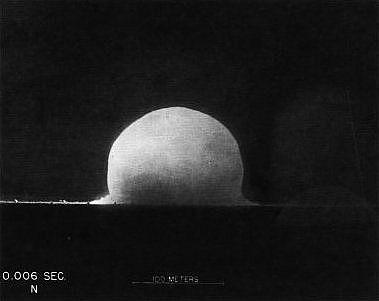
\includegraphics[width=0.9\linewidth]{fig/trinity1.jpg}
  	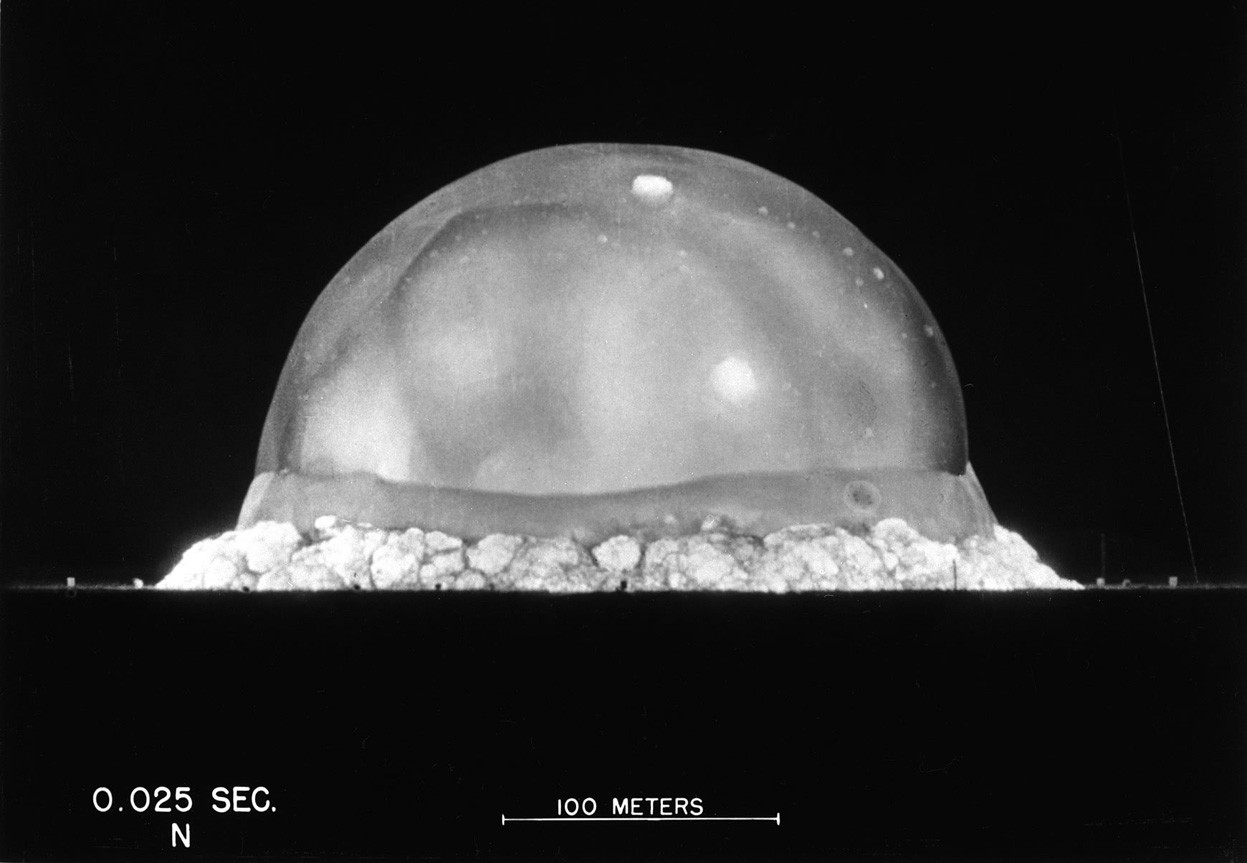
\includegraphics[width=0.9\linewidth]{fig/trinity2.jpg}
  	\caption{Onda de choque del primer ensayo de una bomba atómica denominado \textit{Trinity Test} [1945]. }
  	\label{fig:trinity}
  \end{figure}
 
 Se plantea que la energía liberada $E$ está en función de la densidad del medio $\rho$, el radio de la onda de choque $r$, y el tiempo $t$ desde la detonación. Se desprecian la viscosidad 
 
\begin{table}[htb!]
	\centering
	\begin{tabular}{l||l|lll}
		& $E$ & $t$ & $r$ & $\rho$ \\ \hline
		$L$ & 2   & 0   & 1   & -3     \\ \hline
		$M$ & 1   & 0   & 0   & 1      \\ \hline
		$T$ & -2  & 1   & 0   & 0     
	\end{tabular}
\end{table}
 
\begin{equation*}
	E = t^\alpha r^\beta \rho^\gamma = \begin{cases}
	L:& 2=\beta - 3\rho \\
	M:& 1= \rho \\
	T:& -2 = \gamma
	\end{cases}  
\end{equation*}

Resolviendo el sistema de arriba llegamos a que 
\[E = \frac{\rho r^{5}}{t^{2}} \]
Las dos imágenes en la figura \ref{fig:trinity} son para una explosión de $22$ kT de TNT, equivalente a aproximadamente $10 ^{14}$ joules. Con que certeza se puede calcular la energía de la \textit{Trinity Test}? 






